\documentclass{article}
\usepackage{amsmath} % for the equation* environment
\usepackage{graphicx} % Required for inserting images
\usepackage[margin=1in]{geometry} % sets all margins to 1 inch
\title{Qeueing Theory}
\author{Amine.Bahi }
\date{June 2023}
\usepackage{tikz}
\usepackage{float}
\usepackage{amsmath}
\usepackage{amssymb} % For additional symbols
\usepackage{lipsum} % For sample text; remove this in your actual document


\begin{document}
\maketitle


\section{A Protocol Using Queuing Theory to Hide Volume}

\subsection{Overview Of The M/M/1 Model}

The M/M/1 model is a classic queuing model in which arrivals follow a Poisson distribution, service times are exponentially distributed, and there is a single server. The memoryless property of this model stems from the fact that both inter-arrival and service times are exponentially distributed, making them independent and identically distributed (i.i.d.). The M/M/1 model is characterized by two parameters, the arrival rate ($\lambda$) and the service rate ($\mu$). The performance of the system depends on the relationship between these two parameters, which determines the queue's stability and efficiency.

\paragraph{Applicability and Motivation for Using Queuing Models in Volume-Hiding Schemes}
\label{par:applicability_and_motivation_for_using_queuing models_in_volume-Hiding_schemes}
The motivation to utilize the queuing model arises from the compelling parallels that can be drawn between queuing systems and the challenges faced in volume-hiding structured encryption (VHSTE). A queuing system, such as the M/M/1 or the $M^X/M/1$ model, effectively represents the interaction between demand (arrivals or requests) and supply (server capacity). Similarly, in a VHSTE system, the client demands data (queries) and the server supplies it. Understanding and managing the dynamics of this interaction is crucial to both scenarios.

In the context of VHSTE, the adversary, acting as an eavesdropper, can glean significant insights about the queried data based on the timing and volume of server responses. To counter this, it is necessary to introduce variability in server response times to obfuscate the actual volume of data accessed. This challenge is akin to managing a queuing system where arrival rates, service rates, and service times must be optimally controlled to ensure efficiency while maintaining desired service levels.

Furthermore, the queuing model's inherent memory-less property, resulting from the exponential distribution of inter-arrival and service times, mirrors the desired security attribute in a VHSTE system. The goal is to ensure that each query and response appears independent and random to the observer.

The queuing model also provides a rich set of mathematical and statistical tools for analyzing system performance. Concepts like stability, throughput, and utilization are drawn from queuing theory and can provide valuable insights into the performance and security trade-offs in a VHSTE system.

Lastly, by considering more complex queuing scenarios like the $M^X/M/1$ model, which accommodates batch arrivals, we can better simulate and tackle real-world scenarios.
\paragraph{Volume Hiding in Structured Encryption Using the M/M/1 Queuing Model}

The primary objective of volume-hiding in structured encryption schemes is to obscure the adversary's ability to deduce the volume of data accessed during data retrieval requests. These requests are analogous to arrivals at a service station in queuing theory. For this reason, we find it fitting to interpret our volume-hiding scheme through the lens of the M/M/1 queuing model.

In this model, we consider the incoming request stream as a Poisson process, characterized by an arrival rate, $\lambda$. The server, in turn, services these requests at an average service rate, $\mu$, which necessarily must be greater than $\lambda$ to maintain stability in the queue. An inherent advantage of this model is its memoryless property, which results in response times following an exponential distribution.

\paragraph{Exponential Distribution and its Role in Volume Hiding}

In the context of volume-hiding, the exponential distribution of response times is particularly beneficial as it introduces variability to these times. This variability effectively obfuscates the actual volume of data accessed. To bolster this, we introduce dummy requests or additional delays into the system while maintaining the stability of the queue. This is achieved by ensuring that the effective service rate, which includes both actual and dummy requests, remains higher than the combined rate of arrivals, denoted by $\mu_{\text{effective}} > \lambda + \lambda_{\text{dummies}}$. The dummies are designed to maintain the exponential distribution of response times, thereby fortifying the volume-hiding characteristic of the system.

\paragraph{Complex Queuing Scenarios and the $M^X/M/1$ Model}

However, our model takes a step further by considering a more complex queuing scenario: the $M^X/M/1$ model, which introduces the concept of batch arrivals. Here, queries arrive in batches of varying lengths, making the queue a compound or 'stuttering' Poisson process. The analysis of this model is complex and may not yield a simple closed form. It could require advanced techniques like generating functions and complex analysis, with the specifics depending on the particular distribution of the batch sizes.

\begin{figure}[H]
   \centering
    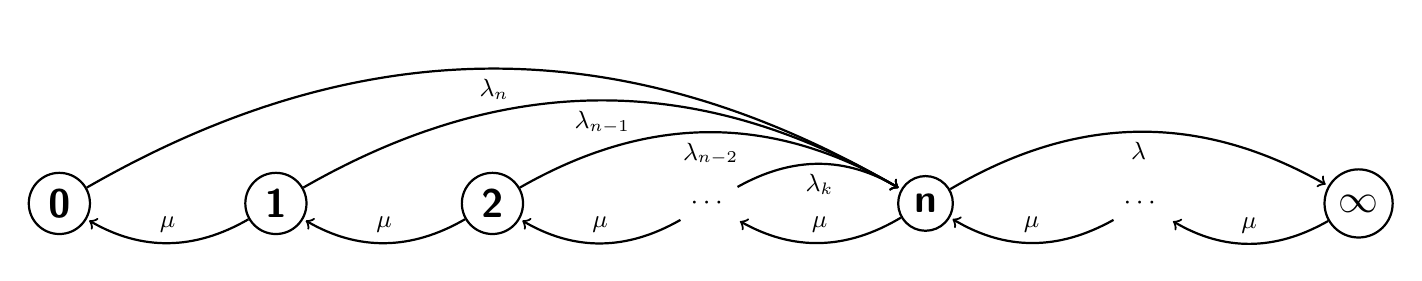
\begin{tikzpicture}[->,shorten >=1pt,auto,node distance=2.75cm, thick, main node/.style={circle,draw,font=\sffamily\Large\bfseries}]
    
      \node[main node] (0) {0};
      \node[main node] (1) [right of=0] {1};
      \node[main node] (2) [right of=1] {2};
      \node (dots1) [right of=2] {$\cdots$};
      \node[main node] (n) [right of=dots1] {n};
      \node (dots2) [right of=n] {$\cdots$};
      \node[main node] (inf) [right of=dots2] {$\infty$};
    
      \path[every node/.style={font=\sffamily\small}]
        (1) edge[bend left] node[above] {$\mu$} (0)
        (2) edge[bend left] node[above] {$\mu$} (1)
        (dots1) edge[bend left] node[above] {$\mu$} (2)
        (n) edge[bend left] node[above] {$\mu$} (dots1)
        (inf) edge[bend left] node[above] {$\mu$} (dots2)
        (dots2) edge[bend left] node[above] {$\mu$} (n);
    
      \path[every node/.style={font=\sffamily\small}]
        (0) edge[bend left] node[below] {$\lambda_n$} (n)
        (1) edge[bend left] node[below] {$\lambda_{n-1}$} (n)
        (2) edge[bend left] node[below] {$\lambda_{n-2}$} (n)
        (dots1) edge[bend left] node[below] {$\lambda_{k}$} (n)
        (n) edge[bend left] node[below] {$\lambda$} (inf);
    \end{tikzpicture}
\caption{Transition rate Diagram from our bulk arrival queue model}
    \label{fig:ctmc}
\end{figure}





In the following, we will delve into specific calculations to derive the exact values of $p_n$, the probability of having $n$ items in the queue. This will involve using the balance equations we establish (\ref{eq:bleq}) and (\ref{eq:b2leq}), from \ref{fig:ctmc} by leveraging the properties of the Poisson arrival and service process. The goal is to arrive at an expression that can effectively be used to determine the queue's behavior under our volume-hiding scheme.




\begin{equation}
\lambda p_0 = \mu p_1\\
\label{eq:bleq}
\end{equation}

\begin{equation}
(\lambda + \mu) p_n = \mu p_{n+1} + \lambda \sum_{k=1}^{n} p_{n-k} c_k; \quad n \geq 1, \quad \text{such that: } \lambda_k = \lambda \times c_k
\label{eq:b2leq}
\end{equation}
We will use the probability-generating function of both queue and batch size $P$ and $C$ respectively:
\begin{equation*}
C(z) = \sum_{n=1}^{\infty} c_n z^n; \quad |z| \leq 1
\end{equation*}

\begin{equation*}
P(z) = \sum_{n=0}^{\infty} p_n z^n; \quad |z| \leq 1
\end{equation*}
We multiply (\ref{eq:b2leq}) by $z^n$ and sum from 1 to $\infty$:

\begin{align*}
&\Rightarrow\lambda \sum_{n=1}^{\infty} p_n z^n + \mu \sum_{n=1}^{\infty} p_n z^n = \frac{\mu}{z} \sum_{n=1}^{\infty} p_{n+1} z^{n+1} + \lambda \sum_{n=1}^{\infty} \sum_{k=1}^{n} p_{n-k} c_k z^n\\
&\Rightarrow\lambda \sum_{n=0}^{\infty} p_n z^n - \lambda p_0 + \mu \sum_{n=1}^{\infty} p_n z^n = \frac{\mu}{z} \sum_{n=2}^{\infty} p_{n} z^{n} + \lambda \sum_{n=1}^{\infty} \sum_{k=1}^{n} p_{n-k} c_k z^n\\
&\Rightarrow\lambda \sum_{n=0}^{\infty} p_n z^n + \mu \sum_{n=1}^{\infty} p_n z^n = \frac{\mu}{z} \sum_{n=0}^{\infty} p_{n} z^{n} -\frac{\mu}{z}p_0 + \lambda \sum_{n=1}^{\infty} \sum_{k=1}^{n} p_{n-k} c_k z^n
\end{align*}

Notice that the 4th term is a convolution of the two PGFs as shown in (\ref{eq:conveq})  :
\begin{equation}
\sum_{n=1}^{\infty} \sum_{k=1}^{n} p_{n-k} c_k z^n = \sum_{k=1}^{\infty} c_k z^k \sum_{n=k}^{\infty} p_{n-k} z^{n-k} = C(z)P(z)
\label{eq:conveq}
\end{equation}

\begin{align*}
\lambda P(z) + \mu [P(z) - p_0] &= \frac{\mu}{z} [P(z) - p_0] + \lambda C(z)P(z)\\
\Rightarrow P(z) &= \frac{\mu (1 - z) p_0}{\mu (1 - z) - \lambda z [1 - C(z)]}; \quad |z| \leq 1\\
\Rightarrow P(z) &= \frac{p_0}{1 - \frac{\lambda z [1 - C(z)]}{\mu [1 - z]}}\\
\Rightarrow P(z) &= \frac{p_0}{1 - \frac{\lambda}{\mu} z \bar{C}(z)}; \quad \text{where: } \bar{C}(z) = \frac{1 - C(z)}{1 - z}\\
\end{align*}
To calculate $p_0$ we will use the fact that $ P(1) = 1$ and l'hopital rule ounce to calculate $\bar{C}(1)$ and let E[X] be the average batch size :
\begin{align*}
p_0 &=1 - \frac{\lambda}{\mu} E[X]\\
&\boxed{p_0 = 1 - \rho}
\end{align*}

\begin{align*}
&P(z) = \frac{(1-\rho)}{1-\frac{\lambda}{\mu} z \bar{C}(z)}\\
&\Rightarrow P(z) - P(z) \frac{\lambda}{\mu} z \bar{C}(z) = p_0\\
&\Rightarrow\sum_{n=0}^{\infty} p_n z^n - P(z) \frac{\lambda}{\mu} z \bar{C}(z) = p_0\\
&\Rightarrow\sum_{n=1}^{\infty} p_n z^n = \frac{\lambda}{\mu} z P(z) \bar{C}(z)\\
&\Rightarrow\sum_{n=1}^{\infty} p_n z^n = \frac{\lambda}{\mu} \sum_{n=0}^{\infty} \sum_{k=0}^{n} p_{n-k} \bar{c}_k z^{n+1}\\
&\Rightarrow\sum_{n=1}^{\infty} p_n z^n = \frac{\lambda}{\mu} \sum_{n=1}^{\infty} \sum_{k=0}^{n-1} p_{n-k-1} \bar{c}_k z^n\\
\end{align*}
\begin{equation*}
\boxed{p_n = \frac{\lambda}{\mu} \sum_{k=0}^{n-1} p_{n-k-1} \bar{c}_k , \quad n \geq 1}
\end{equation*}
We will now attempt to find an upper bound for \( p_n \).\\

We have \(\forall k \in \mathbb{N}\):

\begin{align*}
\bar{c_k} &= 1 - \sum_{i=1}^{k} c_i\\
\bar{c}_{k+1} &= \bar{c_k} - c_{k+1}\\
&=\bar{c_k} \left(1 - \frac{c_{k+1}}{\bar{c_k}} \right)\\
&= \bar{c_k} \cdot \gamma_{k+1}\\
\end{align*}

Since for all \( k \in \mathbb{N^*} \):\\
\[
\gamma_{1} \leq \dots \leq \gamma_{n}
\]

Thus, we now can write :

\begin{align*}
p_n &= \frac{\lambda}{\mu} \sum_{k=0}^{n-1} p_{n-k-1} \bar{c_k}, \quad n \geq 1 \\
&= \frac{\lambda}{\mu} p_{n-1} \bar{c_0} + \frac{\lambda}{\mu} \sum_{k=1}^{n-1} p_{n-k-1} \bar{c_k} \\
&\leq \frac{\lambda}{\mu} p_{n-1} + \gamma_{n} \cdot \frac{\lambda}{\mu} \sum_{k=0}^{n-2} p_{n-1-k-1} \bar{c_k}
\end{align*}

Notice that the second term is \( p_{n-1} \):
\[
p_n \leq \left( \frac{\lambda}{\mu} + \gamma_{n} \right) p_{n-1}
\]
By induction, we can generalize this result to get:
\begin{align*}
&\Rightarrow p_n \leq \left( \frac{\lambda}{\mu} + \gamma_{n} \right)^{n-1} p_1 \\
&\Rightarrow P(X > K) \leq \sum_{k=K}^{\infty} \left( \frac{\lambda}{\mu} + \gamma_{n} \right)^{k-1} p_1
\end{align*}


If we choose \( \frac{\lambda}{\mu} < (1 - \gamma_{n}) \) and use (1) we get:
\begin{align*}
&\boxed{\Rightarrow P\left(X > K\right) \leq \frac{\lambda}{\mu}\cdot\frac{\left( \frac{\lambda}{\mu}+\gamma_{n}\right)^{K-1}}{1-\left(\frac{\lambda}{\mu} + \gamma_{n} \right)}\cdot \left(1-\rho\right)}\\
\end{align*}
\paragraph{Calculating $\gamma$ for Different Distributions}:\\

\textbf{Case 1: Zeta with parameter $s$.}
Let
\begin{align*}
c_{k+1} &= \frac{1}{(k+1)^{s} \zeta(s)}, & \varepsilon_k &= 1 - \frac{H_{k,s}}{\zeta(s)},
\end{align*}
where $H_{k,s}$ is the generalized harmonic number $H_{k,s} = \sum_{i=1}^{k} \frac{1}{i^{s}}$. Then for $k \in \{n, \ldots, n-1\}$ and $\varepsilon_{k+1}$ we have
\begin{align*}
\varepsilon_{k+1} &= 1 - \frac{1}{(k+1)^{s} \zeta(s)} \left( \zeta(s) - H_{k,s} \right) \\
&= 1 - \frac{\zeta(s) - H_{k,s}}{(k+1)^{s}\zeta(s)}.
\end{align*}
From (*) we know that
\begin{align*}
H_{k,s} &> \zeta(s) - k^{1-s} \left( \frac{k}{s-1} + \frac{s}{12k} - \frac{1}{2} \right), \\
\zeta(s) - H_{k,s} &< k^{1-s} \left( \frac{k}{s-1} + \frac{s}{12k} - \frac{1}{2} \right), \\
1 - \frac{\zeta(s) - H_{k,s}}{(k+1)^{s}\zeta(s)} &< 1 - \frac{k^{1-s} \left( \frac{k}{s-1} + \frac{s}{12k} - \frac{1}{2} \right)}{(k+1)^{s}\zeta(s)}, \\
&< 1 - \frac{k^{1-s}}{(k+1)^{s}} \left( \frac{k}{s-1} + \frac{s}{12k} - \frac{1}{2} \right).
\end{align*}
Note that the above quantity is upper-bounded when $k = n - 1$.\\

\textbf{Case 2: Yule-Simon}
\begin{align*}
c_{k+1} &= \rho B(k+1, \rho+1), & \text{where } B(\cdot,\cdot) & \text{ is the beta function}, \\
\gamma_{k+1} &= 1 - \frac{\rho B(k+1, \rho+1)}{B(k, \rho+1)}, & \text{for } k &\in \{0, \ldots, n-1\}.
\end{align*}
We know that
\begin{align*}
B(k+1, \rho+1) &= \frac{k}{k+\rho} B(k, \rho+1),
\end{align*}
then
\begin{align*}
\gamma_{k+1} &= 1 - \frac{\rho \cdot \frac{k}{k+\rho}}{B(k, \rho+1)} = 1 - \frac{\rho}{k+\rho}.
\end{align*}
The above is maximized when \( k = n-1 \). Then
\begin{align*}
\gamma_{k+1} &< 1 - \frac{\rho}{n+\rho}.
\end{align*}

\textbf{Case 3: Uniform}
\begin{align*}
C_k &= 
\begin{cases} 
  \frac{1}{\theta} & \text{if } 0 \leq k \leq \theta, \\
  0 & \text{otherwise},
\end{cases} \\
\gamma_k &= 
\begin{cases} 
  1 - \frac{k}{\theta} & \text{if } 1 \leq k \leq \theta - 1, \\
  0 & \text{otherwise},
\end{cases}
\end{align*}
Note that for $\frac{k}{\theta} > 0$, $c_{k+1} = c_k - \frac{1}{\theta}$ and for $\frac{k}{\theta} \geq 0$ (and hence $\gamma_k \neq 0$) we focus on the case $k < \theta$. We then have
\begin{align*}
\gamma_{k+1} &= \gamma_k \left( 1 - \frac{C_{k+1}}{C_k} \right), \\
\gamma_{k+1} &= 1 - \frac{1/\theta}{1 - k/\theta} = 1 - \frac{1}{\theta - k},
\end{align*}
and its maximum is reached where $k = 0$,
\begin{align*}
\gamma_{k+1} &< 1 - \frac{1}{\theta}.
\end{align*}

In the above cases, the bounds for $p_n$ are obtained as follows:
\begin{align*}
p_n &\leq \left( \frac{\lambda}{\mu} + \gamma_n \right) p_{n-1}, \\
p_{n-1} &\leq \left( \frac{\lambda}{\mu} + \gamma_{n-1} \right) p_{n-2}, \\
\gamma_n &> \gamma_{n-1} \quad \forall n > 0, \\
p_n &\leq \left( \frac{\lambda}{\mu} + \gamma_n \right)^{n-1} p_1.
\end{align*}



\paragraph{Key Metrics in Queuing Theory for Volume Hiding}
In the pursuit of achieving a rigorous understanding of our queue-based volume-hiding scheme, we delve into some fundamental metrics of queuing theory. We have already established two of them: 

\begin{itemize}
    \item \textbf{The utilization factor:} denoted as $\rho$, which signifies the proportion of time the server is busy servicing requests. This is typically computed as the ratio of the arrival rate ($\lambda\cdot E[X]$) to the service rate ($\mu$).

    \item \textbf{The probability distribution of the number of items in the system:}  ($p_n$), which gives us the likelihood of having $n$ items in the system at any given point in time, forms a key component of our analysis.
    
\end{itemize} 
We will now calculate the other crucial ones :
\begin{itemize}
    \item \textbf{The average number of items in the system ($L$):} encompassing both items in the queue and those being serviced.
    \begin{equation*}
    \boxed{L =  P'(1)=\frac{\rho}{1-\rho}\cdot \frac{E[X] + E[X^2]}{2E[X]}}
    \end{equation*}

    \item \textbf{The average waiting time in the system ($W$):} This is intimately related to the average system size ($L$), through Little's Law.
    \item \textbf{The average number of items in the system ($L$):} encompassing both items in the queue and those being serviced.
    \begin{equation*}
    \boxed{L=\left(\lambda\cdot E[X] \right)W}
    \end{equation*}
\end{itemize}
As we proceed, we will explore a more robust model, which is the Bulk servicing model as depicted in \ref{fig:ctmc2}

\begin{figure}[H]
   
    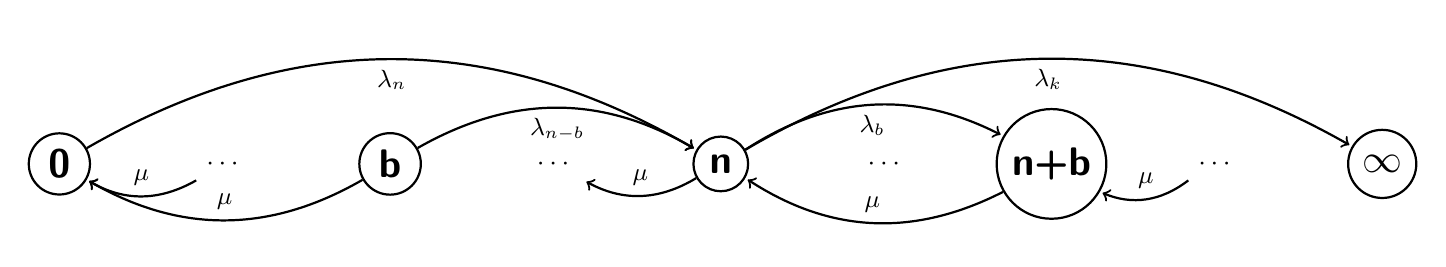
\begin{tikzpicture}[->,,shorten >=1pt,auto,node distance=2.1cm,thick,main node/.style={circle,draw,font=\sffamily\Large\bfseries}]
    
      \node[main node] (0) {0};
      \node (dots0) [right of=0] {$\cdots$};
      \node[main node] (b) [right of=dots0] {b};
      \node (dots1) [right of=b] {$\cdots$};
      \node[main node] (n) [right of=dots1] {n};
      \node (dots2) [right of=n] {$\cdots$};
      \node [main node] (n+b) [right of=dots2] {n+b};
      \node (dots3) [right of=n+b] {$\cdots$};
      \node[main node] (inf) [right of=dots3] {$\infty$};
    
      \path[every node/.style={font=\sffamily\small}]
        (dots0) edge[bend left] node[above] {$\mu$} (0)
        (b) edge[bend left] node[above] {$\mu$} (0)
        (n+b) edge[bend left] node[above] {$\mu$} (n)
        (dots3) edge[bend left] node[above] {$\mu$}  (n+b)
        (n) edge[bend left] node[above] {$\mu$}  (dots1);
        
    
      \path[every node/.style={font=\sffamily\small}]
        (0) edge[bend left] node[below] {$\lambda_n$} (n)
        (b) edge[bend left] node[below] {$\lambda_{n-b}$} (n)
        (n) edge[bend left] node[below] {$\lambda_{k}$} (inf)
        (n) edge[bend left] node[below] {$\lambda_{b}$} (n+b);
        
    \end{tikzpicture}
\caption{Bulk Arrival + Batch servicing Model}
    \label{fig:ctmc2}
\end{figure}


\begin{equation}
\lambda p_0 = \mu p_1 + \mu p_2 + \dots + \mu p_b
\label{eq:bleq3}
\end{equation}
\begin{equation}
(\lambda + \mu)p_n = \mu p_{n+b} + \lambda \sum_{k=1}^{n} p_{n-k} c_k, \quad n \geq 1
\label{eq:b2leq3}
\end{equation}
We will define :
\begin{equation*}
P_b(z) = \sum_{n=0}^{b} p_n z^n; \quad |z| \leq 1
\end{equation*}
We multiply (\ref{eq:b2leq3}) by $z^n$ and sum from 1 to $\infty$:
\begin{align*}
&\Rightarrow(\lambda + \mu) \sum_{n=1}^{\infty} p_n z^n = \frac{\mu}{z^b} \sum_{n=1}^{\infty} p_{n+b} z^{n+b} + \lambda \sum_{n=1}^{\infty} \sum_{k=1}^{n} p_{n-k} c_k z^n\\
&\Rightarrow (\lambda+\mu)\left[\sum_{n=0}^{\infty} p_n z^n - p_0\right] = \frac{\mu}{z^b} \left[\sum_{n=0}^{\infty} p_n z^n - \sum_{n=0}^{b} p_n z^n\right] + \lambda C(z)P(z) \\
&\Rightarrow \lambda P(z) + \mu P(z) - \lambda p_0 - \mu p_0 = \frac{\mu}{z^b} P(z) - \frac{\mu}{z^b} P_b(z) + \lambda C(z)P(z) \\
&\Rightarrow \lambda P(z)[1-C(z)] + \mu P(z) - \mu P_b(1) = \frac{\mu}{z^b} P(z) - \frac{\mu}{z^b} P_b(z) \\
&\Rightarrow \lambda P(z)[1-C(z)] - \mu P(z)\left[\frac{1}{z^b} - 1\right] = \mu P_b(1) - \frac{\mu}{z^b} P_b(z) \\
\end{align*}
We multiply by $z^b$ and divide by $\mu$:
\begin{align*}
\Rightarrow P(z) &= \frac{z^b P_b(1)-P_b(z)}{\frac{\lambda}{\mu} z^b [1 - C(z)] - [1 - z^b]} \\
\Rightarrow P(z) &= \frac{P_b(z) - z^b P_b(1)}{1 -[1+\frac{\lambda}{\mu}] z^b +\frac{\lambda}{\mu} z^b C(z)}\\
\Rightarrow P(z) &= \frac{P_b(z) - z^b P_b(1)}{\left(\sum_{n=0}^{b-1} z^n - \frac{\lambda}{\mu} z^b \bar{C}(z) \right)(1-z)}
\end{align*}
We set $\rho = \frac{\lambda E[X]}{\mu b} < 1$, and define the functions:
\begin{align*}
g(z) &= \sum_{n=0}^{b-1} z^n \\
f(z) &= \frac{\lambda}{\mu} z^b \bar{C}(z) \\
\end{align*}
Both $f$ and $g$  are differentiable in and on the unit circle thus they are analytic.\\
Then, we have: $\frac{f(1)}{g(1)} =\rho < 1 $ \\
We proved $|f(z)| < |g(z)|$, thus Rouché's theorem states that the denominator has exactly $b$ zeros within the unit disk.\\
Thus: $P_b(z) - z^b P_b(1) = A[z - 1][z - z_1] \cdots [z - z_{b-1}]$.\\
\begin{align*}
P(z) &= \frac{P_b(z) - z^b P_b(1)}{\left(\sum_{n=0}^{b-1} z^n - \frac{\lambda}{\mu} z^b \bar{C}(z) \right)(1-z)}  \\
\Rightarrow P(z) &= \frac{-A [z - z_1] \cdots [z - z_{b-1}]}{\sum_{n=0}^{b-1} z^n - \frac{\lambda}{\mu} z^b \bar{C}(z)} \\
\end{align*}
To determine $A$, we'll use $P(1) = 1$.
\begin{align*}
1 &= \frac{-A [1 - z_1] \cdots [1 - z_{b-1}]}{\sum_{n=0}^{b-1} 1 - \frac{\lambda}{\mu} \bar{C}(1)} \\
A &= \frac{\frac{\lambda}{\mu} E[X] - b}{[1 - z_1] \cdots [1 - z_{b-1}]} \\
\end{align*}
We now have:
\begin{align*}
P_b(z) - z^b P_b(1) &= [z - 1]\times\frac{[z - z_1]\cdots [z - z_{b-1}]}{[1 - z_1] \cdots [1 - z_{b-1}]} \times b  \times (\rho -1)\\
\Rightarrow P_b(0) &= p_0 = b  \times (1 - \rho)\times\prod_{i=1}^{b-1} \frac{z_i}{(z_i - 1)} \\
\end{align*}
We can now remark that:
\begin{align*}
P_b(z) - z^b P_b(1) &= [z - 1]\times\prod_{i=1}^{b-1}\frac{z-z_i}{1-z_i}\times b  \times (\rho -1)\\
&\Rightarrow P_b(z) - z^b P_b(1) = [z - 1]\times p_0 b  \times (\rho -1)\times\prod_{i=1}^{b-1}\frac{z_i - z}{z_i}\times \frac{z_i}{z_i-1}\\
&\Rightarrow P_b(z) - z^b P_b(1) =  p_0\times\prod_{i=0}^{b-1}\frac{z - z_i}{z_i}\\
&\Rightarrow P_{b-1}(z) - z^b P_{b-1}(1) = p_0\times\prod_{i=0}^{b-1}\frac{z - z_i}{z_i}\\
\end{align*}
Thus, for $1\leq n \leq b-1 $:
\begin{equation}
\boxed{p_n &= b_np_0} \quad \text{where, $b_n$ are the coefficient of $z^n$ in} \prod_{i=0}^{n}\frac{z - z_i}{z_i}\\
\end{equation}
Comparison, with a multi-server model  as depicted in \ref{fig:ctmc3}

\begin{figure}[H]
   
    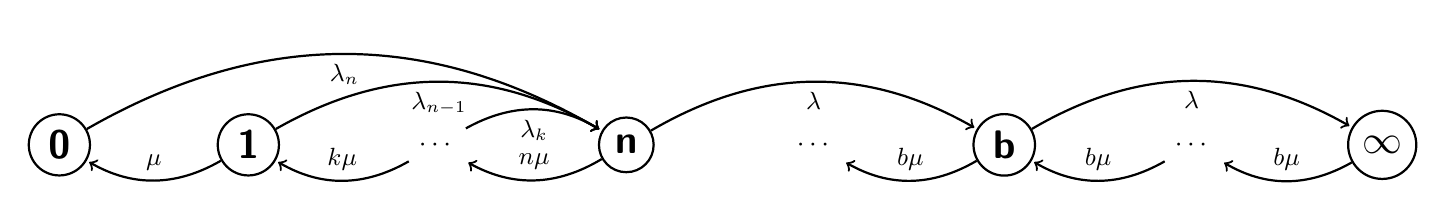
\begin{tikzpicture}[->,,shorten >=1pt,auto,node distance=2.4cm,thick,main node/.style={circle,draw,font=\sffamily\Large\bfseries}]
    
        \node[main node] (0) {0};
        \node[main node] (1) [right of=0] {1};;
        \node (dots1) [right of=1] {$\cdots$};
        \node[main node] (n) [right of=dots1] {n};
        \node (dots2) [right of=n] {$\cdots$};
        \node[main node] (b) [right of=dots2] {b};
        \node (dots3) [right of=b] {$\cdots$};
        \node[main node] (inf) [right of=dots3] {$\infty$};
        
        \path[every node/.style={font=\sffamily\small}]
        (1) edge[bend left] node[above] {$\mu$} (0)
        (dots1) edge[bend left] node[above] {$k\mu$} (1)
        (n) edge[bend left] node[above] {$n\mu$} (dots1)
        (inf) edge[bend left] node[above] {$b\mu$} (dots3)
        (b) edge[bend left] node[above] {$b\mu$} (dots2)
        (dots3) edge[bend left] node[above] {$b\mu$} (b);
        
        
        \path[every node/.style={font=\sffamily\small}]
        (0) edge[bend left] node[below] {$\lambda_n$} (n)
        (1) edge[bend left] node[below] {$\lambda_{n-1}$} (n)
        (dots1) edge[bend left] node[below] {$\lambda_{k}$} (n)
        (n) edge[bend left] node[below] {$\lambda$} (b)
        (b) edge[bend left] node[below] {$\lambda$} (inf);
            

    \end{tikzpicture}
\caption{Bulk Arrival + place c server models}
    \label{fig:ctmc3}
\end{figure}

\begin{equation}
\lambda p_0 = \mu p_1\\
\label{eq:bleq4}
\end{equation}

\begin{equation}
(\lambda + n\mu) p_n = (n+1)\mu p_{n+1} + \lambda \sum_{k=1}^{n} p_{n-k} c_k; \quad b-1 \geq n \geq 1\\
\label{eq:b1leq4}
\end{equation}
\begin{equation}
(\lambda + b\mu) p_n = b\mu p_{n+1} + \lambda \sum_{k=1}^{n} p_{n-k} c_k; \quad n \geq b
\label{eq:b2leq4} 
\end{equation}

We multiply both (\ref{eq:b1leq4} and \ref{eq:b2leq4}) by $z^n$ and sum from 1 to $b-1$ and from b to $\infty$ respectively:
\begin{align*}
\lambda \sum_{n=1}^{b-1} p_n z^n  + \mu \sum_{n=1}^{b-1} np_n z^n   &= \mu z^{-1}\sum_{n=1}^{b-1} (n+1)p_{n+1} z^{n+1} + \lambda \sum_{n=1}^{b-1} \sum_{k=1}^{n} p_{n-k} c_k z^n \\
\lambda \sum_{n=b}^{\infty} p_n z^n + b \mu \sum_{n=b}^{\infty} p_n z^n  &=  b\mu z^{-1} \sum_{n=b}^{\infty} p_{n+1} z^{n+1} + \lambda \sum_{n=b}^{\infty} \sum_{k=1}^{n} p_{n-k} c_k z^n \\
\end{align*}
We sum the 3 equations and get:
\begin{align*}
&\Rightarrow\lambda P(z) + z\mu P_b'(z) + b\mu \sum_{n=b+1}^{\infty} p_n z^n = \mu z^{-1} \left[ \sum_{n=2}^{b} np_n z^n + b\sum_{n=b+1}^{\infty} p_n z^n + zp_1 \right] + \lambda C(z)P(z) \\
&\Rightarrow\lambda P(z)\left[ 1 - C(z) \right] + z\mu P_b'(z) + b\mu \left[ P(z) - \sum_{n=0}^{b} p_n z^n \right] = \mu \left[ \sum_{n=1}^{b} np_n z^{n-1} + b z^{-1} \left(P(z) - \sum_{n=0}^{b} p_n z^n\right) \right] \\ 
&\Rightarrow\lambda P(z)\left[ 1 - C(z) \right] + \mu P_b'(z) \left[ z - 1 \right] + b\mu P(z) \left[ 1 - z^{-1} \right] - b\mu P_b(z) \left[ 1 - z^{-1} \right] = 0 \\
&\Rightarrow z \frac{\lambda}{b\mu} P(z)\left[ 1 - C(z) \right] + P_b'(z) \left[ z - 1 \right] \frac{z}{b} + P(z) \left[ z - 1 \right] - P_b(z) \left[ z - 1 \right] = 0 \\
\end{align*}
\begin{align*}
&\Rightarrow P(z) = \frac{P_b(z) \left[ z - 1 \right] - P_b'(z) \left[ z - 1 \right]\frac{z}{b}}{\left[ z - 1 \right] + z \frac{\lambda}{b\mu} \left[ 1 - C(z) \right]} \\
&\Rightarrow P(z) = \frac{P_b(z) - P_b'(z) \frac{z}{b}}{1 - z \frac{\lambda}{b\mu} \bar{C}(z)} 
\end{align*}
We set $\rho = \frac{\lambda E[X]}{\mu b} < 1$, and define the functions:
\begin{align*}
g(z) &= 1 \\
f(z) &= z \frac{\lambda}{b\mu} \bar{C}(z) \\
\end{align*}
Both $f$ and $g$  are differentiable in and on the unit circle thus they are analytic.\\
Then, we have: $f(1) =\rho < 1 = g(1) $ \\
We proved $|f(z)| < |g(z)|$, thus Rouché's theorem states that the denominator has exactly $0$ zeros within the unit disk.\\
Thus: $P_b(z) - P_b'(z) \frac{z}{b}  = A $.\\
\begin{align*}
P(z) &= \frac{P_b(z) - P_b'(z) \frac{z}{b}}{1 - z \frac{\lambda}{b\mu} \bar{C}(z)} \\
\Rightarrow P(z) &= \frac{A }{1 - z \frac{\lambda}{b\mu} \bar{C}(z)} \\
\end{align*}
To determine $A$, we'll use $P(1) = 1$.
\begin{align*}
1 &= \frac{A}{1 -  \frac{\lambda}{b\mu} \bar{C}(1)}\\
A &= 1-\rho \\
\end{align*}
We now have:
\begin{align*}
&P_b(z) - P_b'(z) = 1-\rho \\
\Rightarrow &P_b(0) = p_0 = 1-\rho \\
\Rightarrow &P(z) =  \frac{1-\rho}{1 -  \frac{\lambda}{b\mu} E[X]
\end{align*}


\section*{Theorem: Batch Latency in a Queue}

\textbf{Theorem}: Let there be a batch of $k$ tokens entering a queuing system with an average service rate of $\mu$. Let $W_q$ denote the average waiting time experienced by a single token from the batch, but not necessarily the first. The total latency $L_k$ for the entire batch is the sum of this waiting time and the collective processing time for all tokens in the batch.

\textit{Formally},
\begin{align*}
L_k =  W_q + \frac{k-1}{2\mu}
\end{align*}

\textbf{Proof}:
1. Regardless of which token in the batch experiences the waiting time $W_q$, it contributes the same amount to the total time for the batch to be processed.
2. Each token has a processing time of $\frac{1}{\mu}$.\\
3. However depending on which token in the batch experiences the waiting time $W_q$ not all tokens must be processed, the latency is $W_q + k' \times \frac{1}{\mu}$.
where $k'$ is the remaining tokens.
4. Combining all the possible configurations the average batch latency is  $L_k = \frac{\sum_{n=0}^{k} \left( W_q + \frac{n}{\mu}\right)}{k} $.\\

Now we will dive into model with no 0 state, we'll keep the same, Bulk arrival with a "never empty queue" 
\begin{figure}[H]
   \centering
    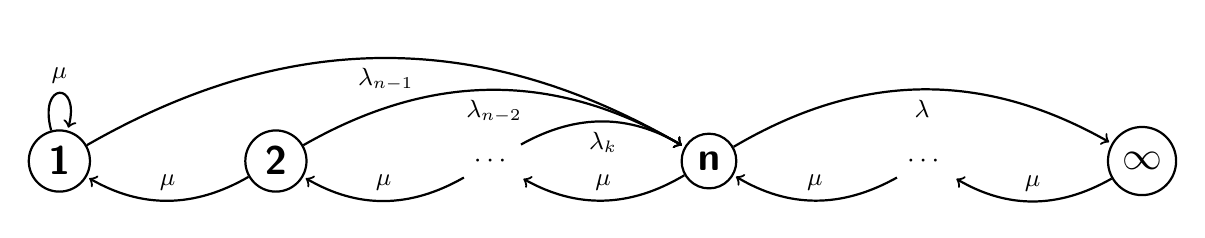
\begin{tikzpicture}[->,shorten >=1pt,auto,node distance=2.75cm, thick, main node/.style={circle,draw,font=\sffamily\Large\bfseries}]
    
      \node[main node] (1) {1};
      \node[main node] (2) [right of=1] {2};
      \node (dots1) [right of=2] {$\cdots$};
      \node[main node] (n) [right of=dots1] {n};
      \node (dots2) [right of=n] {$\cdots$};
      \node[main node] (inf) [right of=dots2] {$\infty$};
    
      \path[every node/.style={font=\sffamily\small}]
        (1) edge[loop above] node[above] {$\mu$} (1)
        (2) edge[bend left] node[above] {$\mu$} (1)
        (dots1) edge[bend left] node[above] {$\mu$} (2)
        (n) edge[bend left] node[above] {$\mu$} (dots1)
        (inf) edge[bend left] node[above] {$\mu$} (dots2)
        (dots2) edge[bend left] node[above] {$\mu$} (n);
    
      \path[every node/.style={font=\sffamily\small}]
        (1) edge[bend left] node[below] {$\lambda_{n-1}$} (n)
        (2) edge[bend left] node[below] {$\lambda_{n-2}$} (n)
        (dots1) edge[bend left] node[below] {$\lambda_{k}$} (n)
        (n) edge[bend left] node[below] {$\lambda$} (inf);
    \end{tikzpicture}
\caption{Transition rate Diagram from our bulk arrival queue model}
    \label{fig:ctmc_dummy}
\end{figure}





In the following, we will delve into specific calculations to derive the exact values of $p_n$, the probability of having $n$ items in the queue. This will involve using the balance equations we establish (\ref{eq:Dbleq}) and (\ref{eq:Db2leq}), from \ref{fig:ctmc_dummy} by leveraging the properties of the Poisson arrival and service process. The goal is to arrive at an expression that can effectively be used to determine the queue's behavior under our volume-hiding scheme.




\begin{equation}
\lambda p_1 + \mu p_1= \mu(p_2 + p_1)\\
\label{eq:Dbleq}
\end{equation}

\begin{equation}
(\lambda + \mu) p_n = \mu p_{n+1} + \lambda \sum_{k=1}^{n-1} p_{n-k} c_k; \quad n \geq 2, \quad \text{such that: } \lambda_k = \lambda \times c_k
\label{eq:Db2leq}
\end{equation}
We will use the probability-generating function of both queue and batch size $P$ and $C$ respectively:
\begin{equation*}
C(z) = \sum_{n=1}^{\infty} c_n z^n; \quad |z| \leq 1
\end{equation*}

\begin{equation*}
P(z) = \sum_{n=0}^{\infty} p_n z^n; \quad |z| \leq 1
\end{equation*}
We multiply (\ref{eq:Db2leq}) by $z^n$ and sum from 2 to $\infty$:

\begin{align*}
&\Rightarrow\lambda \sum_{n=2}^{\infty} p_n z^n + \mu \sum_{n=2}^{\infty} p_n z^n = \frac{\mu}{z} \sum_{n=2}^{\infty} p_{n+1} z^{n+1} + \lambda \sum_{n=2}^{\infty} \sum_{k=1}^{n-1} p_{n-k} c_k z^n\\
&\Rightarrow\lambda \sum_{n=0}^{\infty} p_n z^n - \lambda p_0 - \lambda p_1 z + \mu \sum_{n=2}^{\infty} p_n z^n = \frac{\mu}{z} \sum_{n=3}^{\infty} p_{n} z^{n} + \lambda \sum_{n=2}^{\infty} \sum_{k=1}^{n} p_{n-k} c_k z^n\\
&\Rightarrow\lambda \sum_{n=0}^{\infty} p_n z^n + \mu \sum_{n=2}^{\infty} p_n z^n = \frac{\mu}{z} \sum_{n=0}^{\infty} p_{n} z^{n} -\mu p_1 + \lambda \sum_{n=2}^{\infty} \left[\sum_{k=1}^{n} p_{n-k} c_k z^n- p_0c_nz^n\right]\\
&\Rightarrow\lambda \sum_{n=0}^{\infty} p_n z^n + \mu \sum_{n=0}^{\infty} p_n z^n - \mu p_1 z = \frac{\mu}{z} \sum_{n=0}^{\infty} p_{n} z^{n} -\mu p_1 + \lambda \sum_{n=1}^{\infty}\sum_{k=1}^{n} p_{n-k} c_k z^n
\end{align*}

Notice that the 4th term is a convolution of the two PGFs as shown in (\ref{eq:conveq})  :
\begin{equation}
\sum_{n=1}^{\infty} \sum_{k=1}^{n} p_{n-k} c_k z^n = \sum_{k=1}^{\infty} c_k z^k \sum_{n=k}^{\infty} p_{n-k} z^{n-k} = C(z)P(z)
\label{eq:conveq}
\end{equation}

\begin{align*}
\lambda P(z) + \mu [P(z) - zp_1] &= \frac{\mu}{z} [P(z) - zp_1] + \lambda C(z)P(z)\\
\Rightarrow P(z) &= \frac{\mu (1 - z) zp_1}{\mu (1 - z) - \lambda z [1 - C(z)]}; \quad |z| \leq 1\\
\Rightarrow P(z) &= \frac{zp_1}{1 - \frac{\lambda z [1 - C(z)]}{\mu [1 - z]}}\\
\Rightarrow P(z) &= \frac{zp_1}{1 - \frac{\lambda}{\mu} z \bar{C}(z)}; \quad \text{where: } \bar{C}(z) = \frac{1 - C(z)}{1 - z}\\
\end{align*}
To calculate $p_0$ we will use the fact that $ P(1) = 1$ and l'hopital rule ounce to calculate $\bar{C}(1)$ and let E[X] be the average batch size :
\begin{align*}
1\cdot p_1 &=1 - \frac{\lambda}{\mu} E[X]\\
&\boxed{p_1 = 1 - \rho}
\end{align*}

\begin{align*}
&P(z) = \frac{z(1-\rho)}{1-\frac{\lambda}{\mu} z \bar{C}(z)}\\
&\Rightarrow P(z) - P(z) \frac{\lambda}{\mu} z \bar{C}(z) = zp_1\\
&\Rightarrow\sum_{n=0}^{\infty} p_n z^n - P(z) \frac{\lambda}{\mu} z \bar{C}(z) = zp_1\\
&\Rightarrow\sum_{n=2}^{\infty} p_n z^n = \frac{\lambda}{\mu} z P(z) \bar{C}(z)\\
&\Rightarrow\sum_{n=2}^{\infty} p_n z^n = \frac{\lambda}{\mu} \sum_{n=1}^{\infty} \sum_{k=0}^{n} p_{n-k} \bar{c}_k z^{n+1}\\
&\Rightarrow\sum_{n=2}^{\infty} p_n z^n = \frac{\lambda}{\mu} \sum_{n=2}^{\infty} \sum_{k=0}^{n-1} p_{n-k-1} \bar{c}_k z^n\\
\end{align*}
\begin{equation*}
\boxed{p_n = \frac{\lambda}{\mu} \sum_{k=0}^{n-1} p_{n-k-1} \bar{c}_k , \quad n \geq 2}
\end{equation*}
\end{document}
